Within this section, we will analyze the system's physical modeling. We will derive a physical model of the system using Lagrangian mechanics, which involves defining the kinetic and potential energies of the system, and applying the Euler-Lagrange equation to obtain the equations of motion.
The Lagrangian \( L \) is defined as the difference between the kinetic energy \( T \) and potential energy \( V \) of the system:
\begin{equation}
    L = T - V
    \label{eq:lagrangian}
\end{equation}

The Lagrange's equation in generalized coordinates is given by
\begin{equation}
    \frac{d}{dt} \left( \frac{\partial L}{\partial \dot{q}_i} \right) - \frac{\partial L}{\partial q_i} = 0
    \label{eq:lagrange_equation_equals_zero}
\end{equation}
where \( q_i \) are the generalized coordinates, \( \dot{q}_i \) are the generalized velocities.\cite{widnall:2009}
We will use this framework to derive the equations of motion for the pendulum system, taking into account the forces acting on it, including gravitational forces and the torque generated by the motor.
The final form of the Lagrange's equation we will be using to derive the equations of motion for our pendulum system is given by adding the generalized forces \( Q_i \) to the right-hand side of \eqref{eq:lagrange_equation_equals_zero}:
\begin{equation}
    \frac{d}{dt} \left( \frac{\partial L}{\partial \dot{q}_i} \right) - \frac{\partial L}{\partial q_i} = Q_i
    \label{eq:lagrange_equation}
\end{equation}
Where \( Q_i \) represents the generalized forces acting on the system. Which in our case will include the torque generated by the propeller, frictional forces, and any other external forces acting on the pendulum.

\subsection{Physical Modeling}
%% TODO: write the process of deriving the physical model using Lagrangian mechanics
Derive the physical model of the pendulum system using Lagrangian mechanics, starting from defining the kinetic and potential energies of the system, and applying the Euler-Lagrange equation to obtain the equations of motion.

TODO: CONTINUE FROM HERE...

\subsection{Frictions}
All the frictional forces acting on the pendulum can be modeled as torques opposing the motion of the pendulum, thus we will be adding them along side the other generalized forces \( Q_i \) in \eqref{eq:lagrange_equation}.
Within the friction models, we will always consider the direction of the angular velocity \( \dot{\theta} \) to determine the direction of the frictional torque using the smooth continues function hyperbolic tangent (\(\tanh\)), because of the near zero continuity it provides.
The models will always negate the frictional torque to oppose the motion of the pendulum, thus meaning we will always have a negative sign as the first operator in the modeled friction.

\subsubsection{Viscous Friction}
Viscous friction is a force that opposes the motion of the pendulum and is proportional to its angular velocity and is linear. Allowing for the use of this friction when a linearized model of the system is considered. It can be modeled as:
\begin{equation}
    \tau_{viscous} = -\beta \dot{\theta}
    \label{eq:viscous_friction}
\end{equation}
where \( \tau_{viscous} \) is the viscous friction torque, \( \beta \) is the viscous friction coefficient, and \( \dot{\theta} \) is the angular velocity of the pendulum.

\subsubsection{Coulomb Friction}
Otherwise known as dry friction.
Coulomb friction is a constant force that opposes the motion of the pendulum, regardless of its velocity. It can be modeled as:
\begin{equation}
    \tau_{coulomb} = -\tau_c \tanh(k_c \dot{\theta})
    \label{eq:coulomb_friction}
\end{equation}
where \( \tau_{coulomb} \) is the Coulomb friction torque, \( \tau_c \) is the Coulomb friction coefficient, and \( \tanh(k_c \dot{\theta}) \) is the hyperbolic tangent function of the angular velocity to smooth the transition near zero velocity, $k_c$ is the smoothing coefficient.
We adopt an approach with the hyperbolic tangent function to avoid discontinuities in the model at zero velocity and possible noise induced chattering effects when observing the velocity state of the system.
Equation \eqref{eq:coulomb_friction} can be rewritten into the following form, where we force an interaction between the Coloumb friction and Sticky friction models
\begin{equation}
    \tau_{coulomb} = -\tau_c \tanh(h_c \frac{\dot{\theta}}{\dot{\theta}_{dry}})
    \label{eq:coulomb_friction_modified}
\end{equation}
where \( h_c \) is the modified smoothing coefficient for Coulomb friction, and \( \dot{\theta}_{dry} \) is the dry angular velocity threshold, which can be further defined as
\begin{equation}
    \dot{\theta}_{dry} = \frac{\dot{\theta}_{brk}}{10}
    \label{eq:dry_velocity}
\end{equation}
where \( \dot{\theta}_{brk} \) is the breakaway angular velocity threshold used to define the Stribeck angular velocity in \eqref{eq:stribeck_velocity}, thus creating a relation between the two friction models.

\subsubsection{Sticky Friction}
Otherwise known as adhesion friction. Sticky friction is a force that opposes the initiation of motion when the pendulum is at rest. It can be modeled as:
\begin{align}
    \tau_{sticky} &= -\sqrt{2 e} (\tau_{brk} - \tau_{coulomb}) \exp \left(-\left[ \frac{\dot{\theta}}{\dot{\theta}_{S}} \right]^2\right)  \frac{\dot{\theta}}{\dot{\theta}_{S}} \\
    \tau_{sticky} &= - k_s \exp \left(-\left[ \frac{\dot{\theta}}{\dot{\theta}_{S}} \right]^2\right)  \frac{\dot{\theta}}{\dot{\theta}_{S}}
    \label{eq:sticky_friction}
\end{align}
where \( \tau_{sticky} \) is the sticky friction torque, \( e \) is the Euler number approximation, \( \tau_{brk} \) is the breakaway friction torque, \( \tau_{coulomb} \) is the Coulomb friction torque, \( \dot{\theta}_{S} \) is the Stribeck angular velocity threshold, and \( k_s = \sqrt{2 e} (\tau_{brk} - \tau_{coulomb}) \) is the sticky friction coefficient.\cite{altpeter:1999,de2000control}
The Stribeck effect describes the phenomenon where the frictional force decreases as the velocity of the pendulum increases from rest, reaching a minimum at a certain velocity before transitioning to Coulomb friction at higher velocities.
Stribeck angular velocity threshold \( \dot{\theta}_{S} \) defines the velocity at which this transition occurs and can be defined as follows
\begin{equation}
    \dot{\theta}_{S} = \dot{\theta}_{brk}\sqrt{2}
    \label{eq:stribeck_velocity}
\end{equation}
where \( \dot{\theta}_{brk} \) is the breakaway angular velocity threshold, which defines the velocity at which the breakaway friction transitions to Coulomb friction and can be determined experimentally, or estimated based on the system's characteristics.

\subsubsection{Air Resistance}
Air resistance is a force that opposes the motion of the pendulum due to the drag caused by air, also called the drag force. It can be modeled as:
\begin{equation}
    \tau_{air} = -\frac{1}{2} C_d \rho A r^2 |\dot{\theta}| \dot{\theta}
    \label{eq:air_resistance}
\end{equation}
where \( \tau_{air} \) is the air resistance torque, \( C_d \) is the drag coefficient, \( \rho \) is the air density, \( A \) is the cross-sectional area of the pendulum, \( r \) is the distance from the pivot point to the center of mass, and \( \dot{\theta} \) is the angular velocity of the pendulum.\cite{Benson_1999}
In this model, the air resistance torque is proportional to the square of the angular velocity, thus we include the absolute value of the angular velocity \( |\dot{\theta}| \) to ensure that the torque always opposes the motion of the pendulum, without needing to rely on the hyperbolic tangent function.
We will further simplify \eqref{eq:air_resistance} to a form proportional to the square of the angular velocity for easier integration into our model. Thus, we can rewrite it as:
\begin{equation}
    \tau_{air} = -k_a \dot{\theta}^2 \tanh(k_r \dot{\theta})
    \label{eq:air_resistance_simplified}
\end{equation}
where \( k_a \) is the air resistance coefficient, \( k_r \) is the smoothing coefficient and \( \dot{\theta} \) is the angular velocity of the pendulum.
\newline

Finally, the total friction torque \( \tau_{friction} \) acting on the pendulum can be expressed as the sum of all the individual friction torques:
\begin{align}
    \tau_{friction} &= \tau_{viscous} + \tau_{coulomb} + \tau_{sticky} + \tau_{air} \label{eq:total_friction_general} \\
    \tau_{friction} &= -\beta \dot{\theta} - \tau_c \tanh(k_c \dot{\theta}) - k_s \exp \left(-\left[ \frac{\dot{\theta}}{\dot{\theta}_{brk}} \right]^2\right)  \frac{\dot{\theta}}{\dot{\theta}_{brk}} - k_a \dot{\theta}^2 \tanh(k_r \dot{\theta})
    \label{eq:total_friction}
\end{align}
equation \eqref{eq:total_friction} will be used in our modeling of the pendulum system by including it in the generalized forces \( Q_i \) in the Lagrange equation \eqref{eq:lagrange_equation}. The modeled friction will help us better represent the real-world behavior of the pendulum system, accounting for energy losses due to frictional forces acting on the system.
A simple preview of the friction model behavior can be seen in \figref{fig:friction_model_preview}, where we plot the total friction torque \( \tau_{friction} \) as a function of angular velocity \( \dot{\theta} \) using example coefficients for each friction type.

\begin{center}
    \vbox{
        \makebox[0.5\textwidth][c]{%
        %% TODO: change the plot to matlab figure
            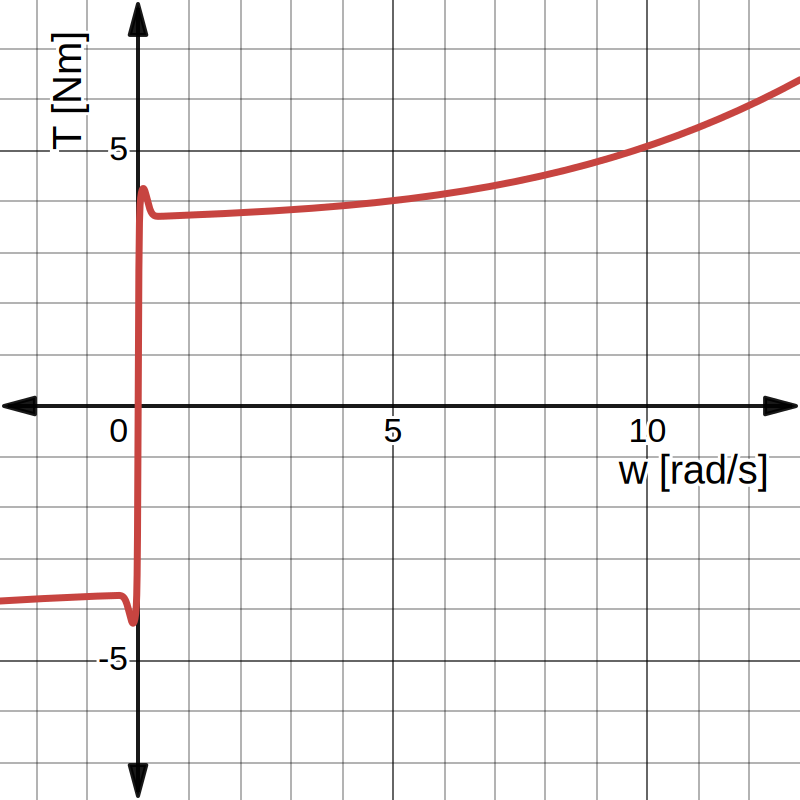
\includegraphics[width=0.4\textwidth]{img/frictions_modeled.pdf}
        }

        \figcaption{
            Plotted preview of the total friction torque \( \tau_{friction} \) as a function of angular velocity \( \dot{\theta} \) using example coefficients for each friction type.
        }
        \label{fig:friction_model_preview}
    }%vbox
\end{center}

The coefficients used in the preview plot are as follows:
\begin{center}
    \vspace{-10pt}

    \tabcaption{Example coefficient values used in friction model preview}
    \label{tab:example_friction_coefficients}
    \begin{tabular*}{\textwidth}{@{ \extracolsep{\fill}} lll}
        \toprule
        Coefficient & Value & Unit \\
        \midrule
        $\beta$ & $0.04$ & $\left[\frac{Nm}{rad/s}\right]$ \\
        $k_a$ & $0.1$ & $\left[\frac{Nm}{rad^2/s^2}\right]$ \\
        $k_r$ & $0.01$ & $\left[\frac{1}{rad/s}\right]$ \\
        $k_c$ & $1000$ & $\left[\frac{1}{rad/s}\right]$ \\
        $\tau_c$ & $3.7$ & $[Nm]$ \\
        $k_s$ & $3.14$ & $[Nm]$ \\
        $\dot{\theta}_{brk}$ & $0.1$ & $[rad/s]$ \\
        $\tau_{brk}$ & $5.05$ & $[Nm]$ \\
        \bottomrule
    \end{tabular*}
\end{center}

\subsection{Modeling Physical Angular Constraints}
Represent the physical angular constraints of the pendulum within the derived model? Or simply note that they exist but will not be modeled directly. But modeled separately in simulation as a stiff spring-damper system at the limits? Or by simply inversing the velocity with a damping factor when the limits are hit?